\documentclass[border=4pt]{standalone}
\usepackage[utf8]{inputenc}
\usepackage[T1]{fontenc}
\usepackage{lmodern}
\usepackage{amsmath,amssymb,mathtools}
\usepackage{tikz}
\usetikzlibrary{calc,decorations.pathreplacing,angles,quotes}
\usepackage{pgfplots}
\pgfplotsset{compat=1.18}
% Figura extraída de la Tarea 11 de Cálculo I (primer semestre).
\begin{document}
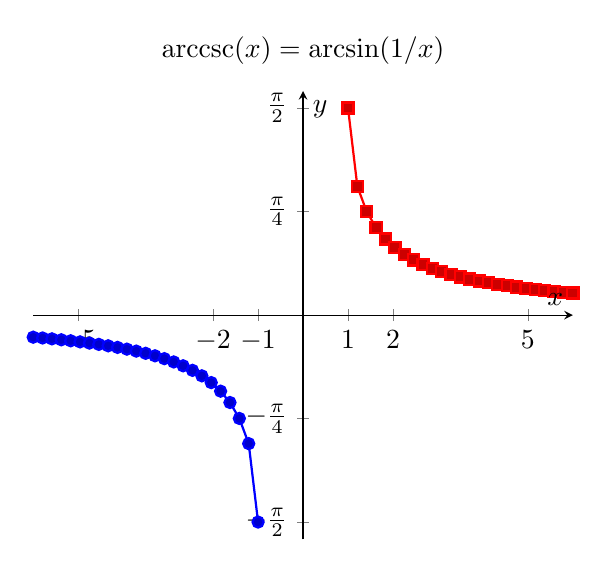
\begin{tikzpicture}
        \begin{axis}[
        xmin=-6,xmax=6,ymin=-1.7,ymax=1.7,
        axis lines=middle,xlabel={$x$},ylabel={$y$},
        xtick={-5,-2,-1,1,2,5},
        ytick={-1.5708,-0.7854,0,0.7854,1.5708},
        yticklabels={\(-\tfrac{\pi}{2}\),\(-\tfrac{\pi}{4}\),0,\(\tfrac{\pi}{4}\),\(\tfrac{\pi}{2}\)},
        title={\(\operatorname{arccsc}(x)=\arcsin(1/x)\)}
        ]
        \addplot+[thick,domain=-6:-1]{asin(1/x)*pi/180};
        \addplot+[thick,domain=1:6]{asin(1/x)*pi/180};
        \end{axis}
    \end{tikzpicture}
\end{document}
